
\section{Simulation}
\label{sec:simulation}

\par  With the circuit solved using the mesh and node methods, it's necesssary to solve it experimentally. In order to simulate the real conditions, which we would have encountered in the laboratory, Ngspice was used. The results obtained from this simulation will take in account the energy dissipation due to the many processes that occur such as Joule effect on conductors. Using this software, we were able to verify the results obtained from the methods already described. 

\par  In order to describe the circuit to be studied, it is necessary to follow some guidelines. Firstly, it was needed to specify , for each component, which were its positive and negative nodes. Because of that, the current directions were defined accordingly to the picture shown. As such, the electric resistances, current sources and the capacitor are going to have the positive node in the location of the current input and the negative node in the current output. The voltage sources nodes were defined so that the nodes are in accordance with the pre established nodes.  the picture below, a brief representation of the interpertation of the circuit by the ngspice programme is presented.

\par Apart from this, it was also necessary to establish the values of the resistance, current and voltage associated with the resistors and independent current and voltage sources. The dependent sources, Vc and Ib (Hc and Gb in ngspice because of the symbolic representation in the program), were respectively current controlled voltage source and voltage controlled current source. Because of that, kc and kb were in kOhm and mS as the script indicated. In the case of Vc, it was needed to indicate a control voltage source, Ve which, even though it doesn't exist, is going to measure the current Ic, the control current, passing through it. This voltage control has a null potential so it doesn't interfere with the rest of the circuit. The nodes of Ve were placed in the circuit so that the current input is in the positive node of the voltage source and the output of the current is in the negative node of the source.  In the case of Ib, it was needed to introduce the nodes in which the potential difference is going to be read (again the positive node in first place and then the negative one).

\par For the first point, it is asked to simulate the circuit when t is less than zero. As such, $vs=Vs$ and the current is DC, which means that there is no voltage variation with time in nodes 0 and 1 and, as the other sources are linear, voltage won't varie with time in the nodes. As such, the current which passes through the capacitor is going to be null as there is no variation with the potential difference in it. Runing the simulation (not transient as all intensity and potential values are constant), we obtain a table with the values of the current and voltage in all nodes confirming what was previously said. This confirmes the values calculated through octave in the theoretical analysis. Below a table with the values obtained and the errors associated is shown.

\vspace{5mm}
\begin{table}[H]
\centering
\begin{tabularx}{0.6\textwidth} {
  | >{\raggedright\arraybackslash}X
  | >{\raggedleft\arraybackslash}X | }
 \hline
@ca[i] & 0.000000e+00\\ \hline
@gb[i] & -2.68449e-04\\ \hline
@r1[i] & 2.563813e-04\\ \hline
@r2[i] & -2.68449e-04\\ \hline
@r3[i] & -1.20678e-05\\ \hline
@r4[i] & 1.186012e-03\\ \hline
@r5[i] & -2.68449e-04\\ \hline
@r6[i] & 9.296302e-04\\ \hline
@r7[i] & 9.296302e-04\\ \hline
v(1) & 5.125559e+00\\ \hline
v(2) & 4.861047e+00\\ \hline
v(3) & 4.313554e+00\\ \hline
v(5) & 4.898549e+00\\ \hline
v(6) & 5.710299e+00\\ \hline
v(7) & -1.91255e+00\\ \hline
v(8) & -2.87912e+00\\ \hline
v(9) & -1.91255e+00\\ \hline

\end{tabularx}
\end{table}
\vspace{5mm}

\par With the natural response values obtained, it's now asked to simulate the natural and forced response on node 6 now with vs as given in the script. The natural solution, as it doesn't varie with the values of the source in the circuit will be the same in this and the previous case. The forced solution is equivelent to the response of the node when vs is applied to the circuit maintining the condition that initially the values of the voltages in nodes 6 and 8 were the ones calculated in point 2 of the simulation (in order to simplify the code the values used were the ones calculated through octave in question 2). As the values in the nodes at the beggining of the transient simulation aren't the ones in which the circuit is stable, variation of the potential difference through the capacitor is going to happen. This can be seen in the ploted graph in which, v(1) varies around 0V as it is connected to the source and v(6) starts at near 6V and after 20ms is also varying around 0V. Also, as the voltage source response is given by a sinusoidal function, regular variation of the voltage in all the nodes is going to appear as also in them voltage values are given by sinusoidal funtions with the same given frequency (but different amplitudes). As seen in the graph below, regular oscilation can be seen in V(6) and v(1) even though the circuit has stabelized after 20ms.
\par All of this means that, variation of the potential difference through the capacitor is going to be noticeable and current isn't null. Notice that the amplitude of the current source vs is 1 and as seen in the graph amplitude is also 1 in v(1). However, the amplitude of voltage in node 6 is no longer 1 (approx 0.8V) as voltage is loss in the rest of the components of the circuit until the current reaches node 6. 

\begin{figure}[h] \centering
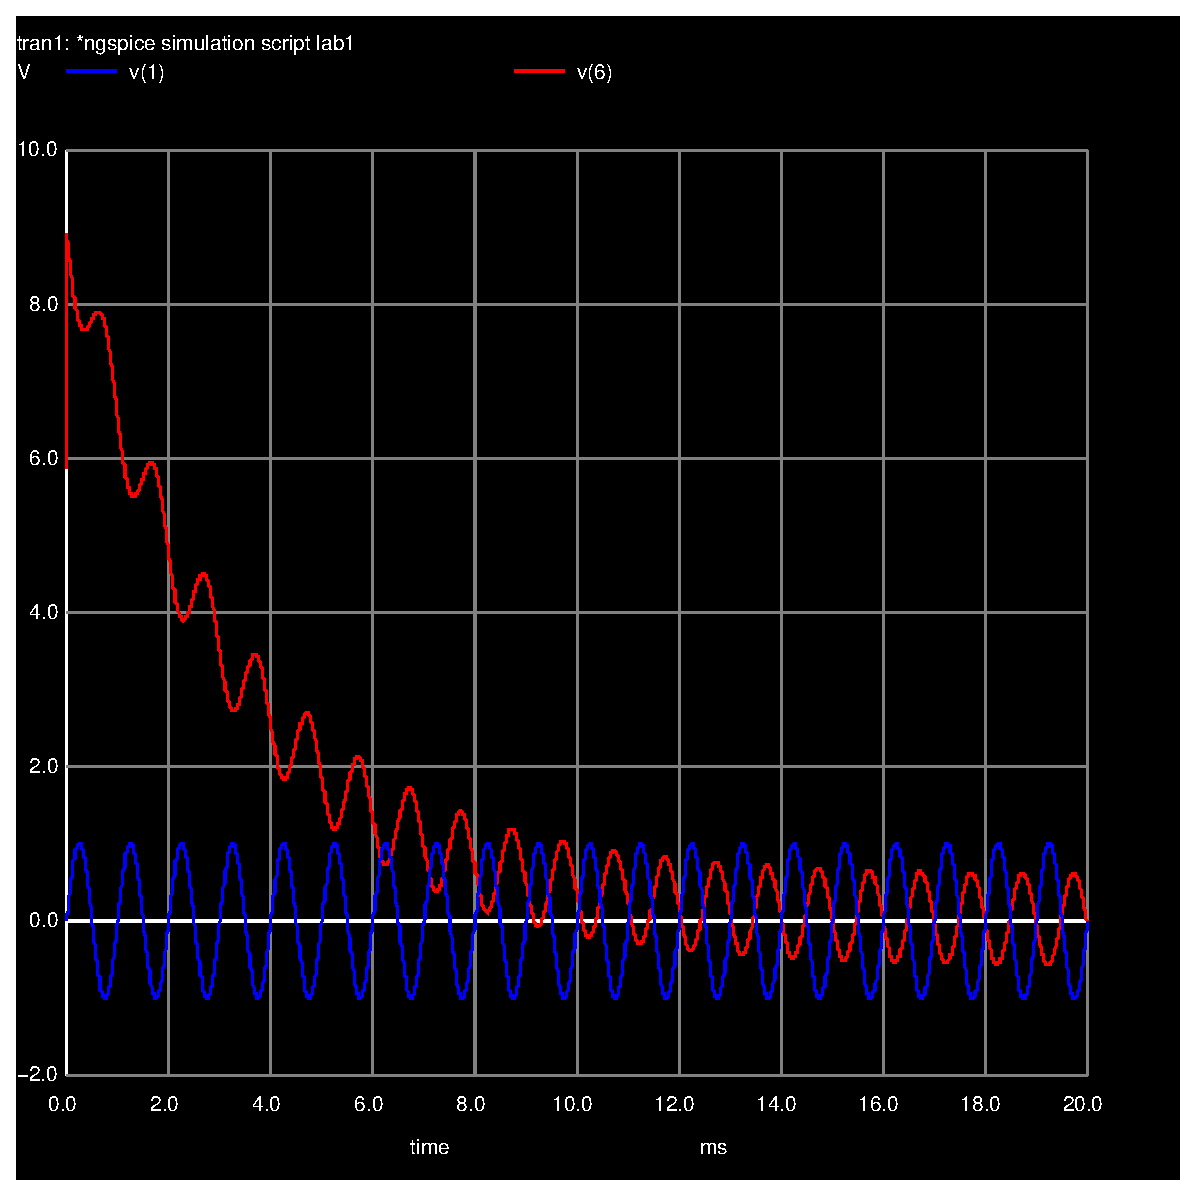
\includegraphics[width=0.6\linewidth]{teste_4.ps}
\caption{Voltages as functions of time}
\label{fig:V(t)}
\end{figure}

\par Finally, in the last question it was studied the frequency response in node 6 through the plot of the phase (rad) in function of the frequency and the magnitude in decibels (in which a 20db increment corresponds to 10x more amplitude) in function of the frequecy of the voltage source and thus the frequecy of the circuit. In these plots a logarithmic scale was used so that the graphics could be read more easily. 

\begin{figure}[h] \centering
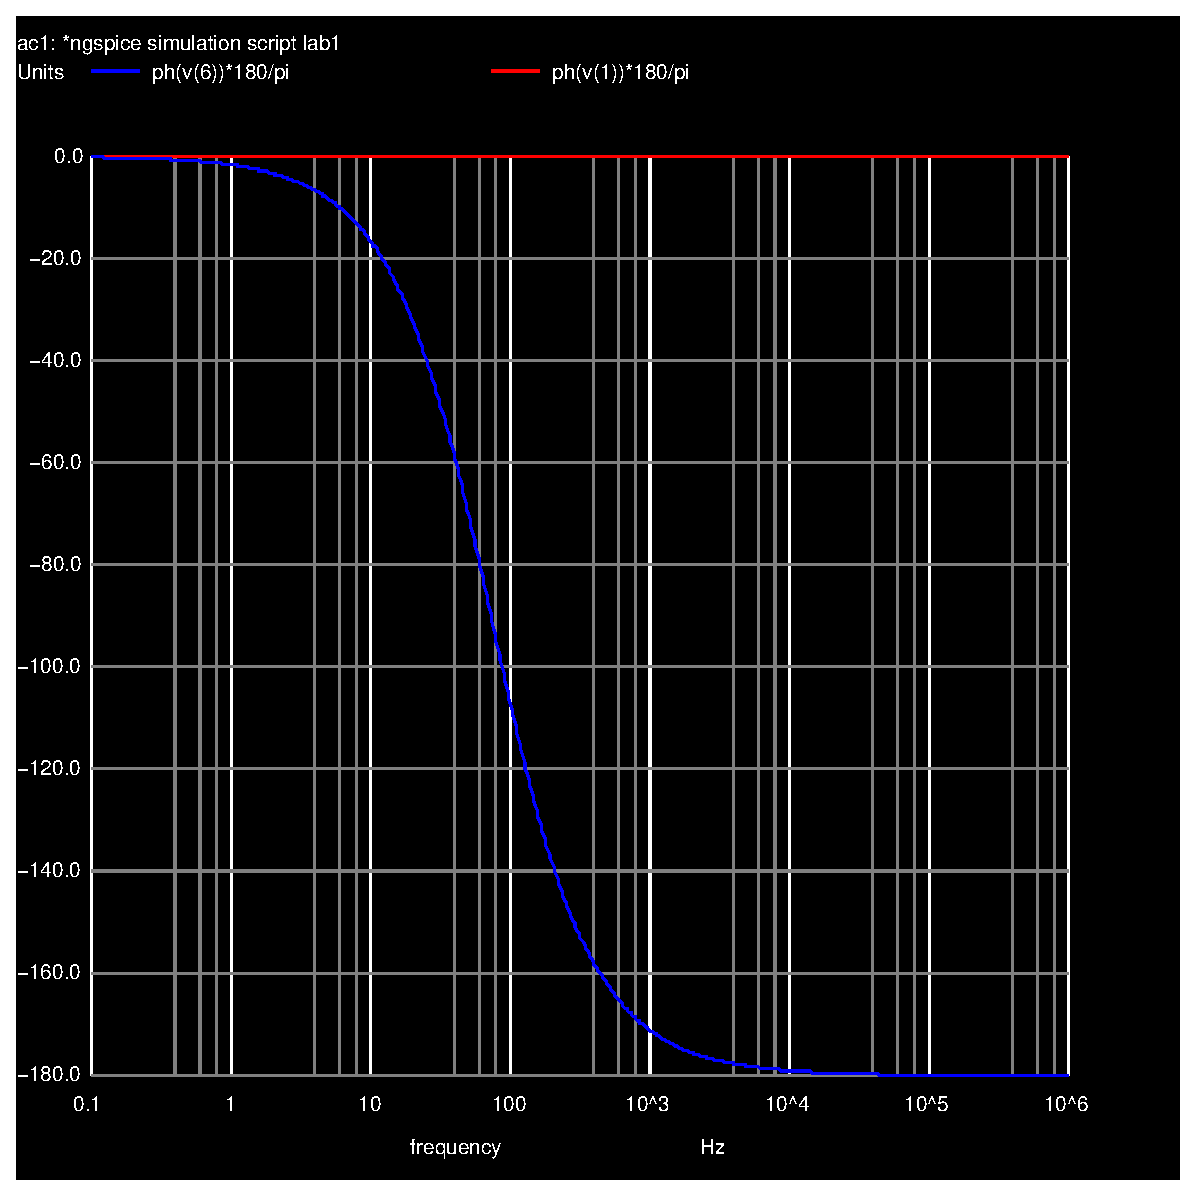
\includegraphics[width=0.6\linewidth]{teste_5_p.ps}
\caption{Phase as function of frequency}
\label{fig:Ph(v(1))*180/pi Ph(v(6))*180/pi}
\end{figure}

\begin{figure}[h] \centering
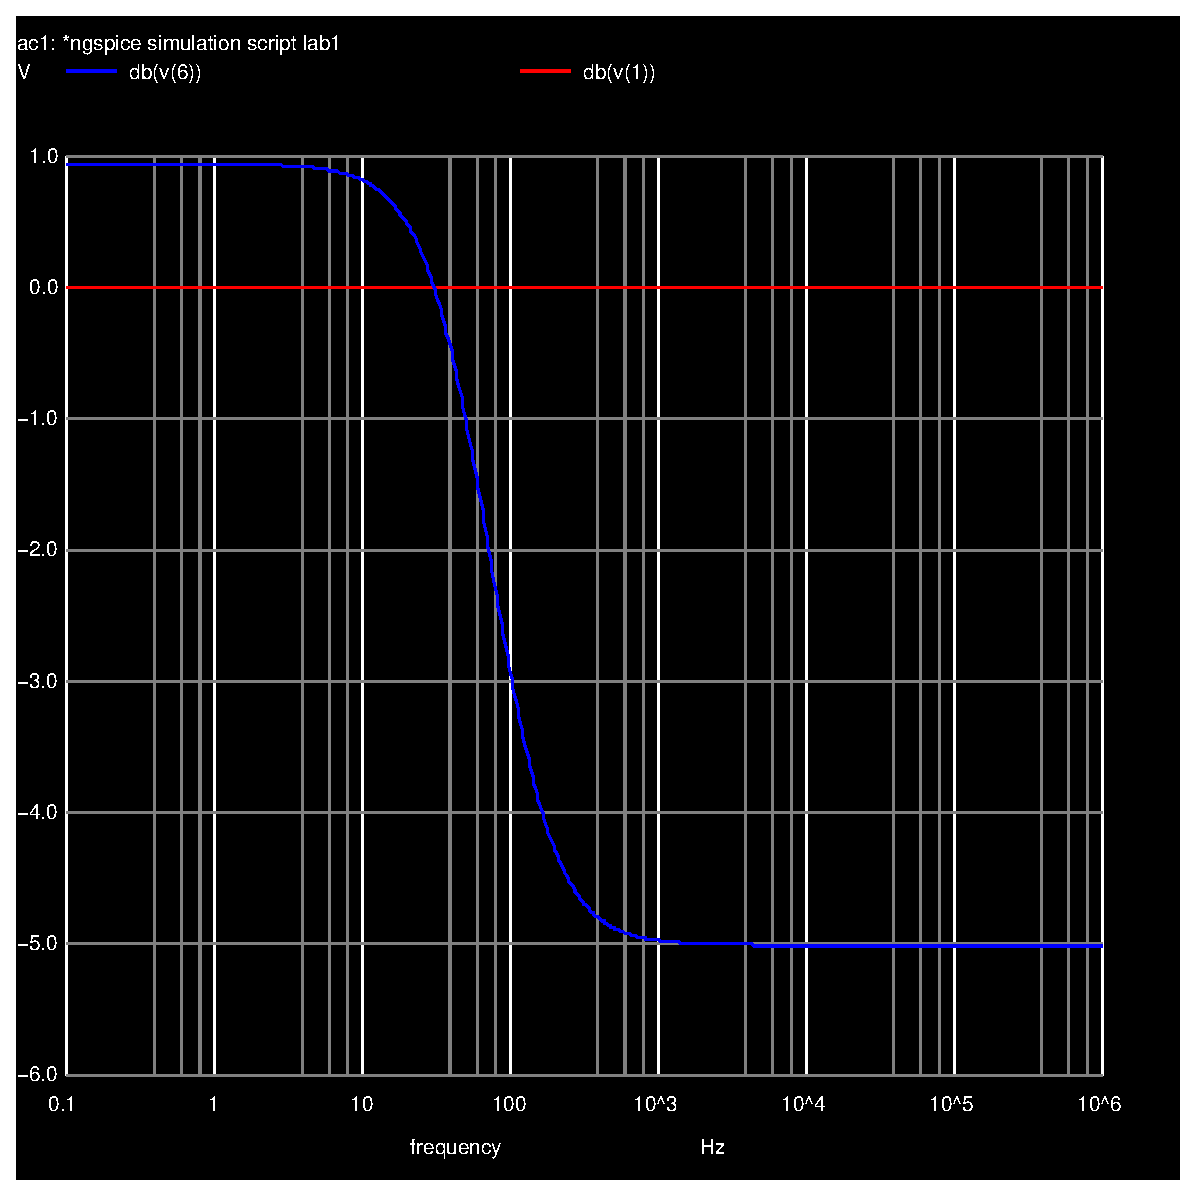
\includegraphics[width=0.6\linewidth]{teste_5_db.ps}
\caption{Voltage magnitude as function of time}
\label{fig:db(v(1)) db(v(6))}
\end{figure}

\par In the first graphic which describes the phase of v(1) and v(6), as given by the expression intially given of v(1) when t>0, its phase is null independently of the value of frequency.  As we can see, the same doesn't happen to the phase of node 6. The reason why this happens can be seen in \ref{analysis.tex}.

\par In the second graphic, the magnitude is expressed in db. In this case, the magnitude of V(1) is constant and null as its magnitude is always 1V and $log(1)=0$. In the case of the magnitude of v(6) as we can see in the equation below, its magnitude varies. The reason why this happens can be seen in \ref{analysis.tex}. 


 
